% Created 2016-04-25 Mon 23:49
\documentclass[11pt]{article}
\usepackage[utf8]{inputenc}
\usepackage{lmodern}
\usepackage[T1]{fontenc}
\usepackage{fixltx2e}
\usepackage{graphicx}
\usepackage{longtable}
\usepackage{float}
\usepackage{wrapfig}
\usepackage{rotating}
\usepackage[normalem]{ulem}
\usepackage{amsmath}
\usepackage{textcomp}
\usepackage{marvosym}
\usepackage{wasysym}
\usepackage{amssymb}
\usepackage{amsmath}
\usepackage[version=3]{mhchem}
\usepackage[numbers,super,sort&compress]{natbib}
\usepackage{natmove}
\usepackage{url}
\usepackage{minted}
\usepackage{underscore}
\usepackage[linktocpage,pdfstartview=FitH,colorlinks,
linkcolor=blue,anchorcolor=blue,
citecolor=blue,filecolor=blue,menucolor=blue,urlcolor=blue]{hyperref}
\usepackage{attachfile}
\usepackage{siunitx}
\usepackage[left=1in, right=1in, top=1in, bottom=1in, nohead]{geometry}
\geometry{margin=1.0in}
\usemintedstyle{emacs}
\newminted{python}{fontsize=\normalsize}
\usepackage{framed,color}
\definecolor{shadecolor}{rgb}{1.0,0.8,0.3}
\author{William F. Schneider}
\date{\today}
\title{Lecture Notes for CBE 20255}
\begin{document}

\begin{options}
\end{options}

\section{Introduction to Engineering Calculation}
\label{sec-1}
\begin{itemize}
\item Base units
\end{itemize}

\begin{center}
\begin{tabular}{llll}
\hline
Dimension & SI & cgs & English\\
\hline
Length & m & cm & in, ft, mi\\
Mass & kg & g & lb$_{\text{m}}$\\
Time & s & s & s\\
Temperature & K & K & F\\
Current & A & A & \\
Light intensity & cd & cd & \\
\hline
\end{tabular}
\end{center}

\begin{itemize}
\item Derived units
\end{itemize}
\begin{center}
\begin{tabular}{llll}
\hline
Volume & liter & L & 1000 cm$^{\text{3}}$\\
Force & Newton & N & 1 kg m/s$^{\text{2}}$\\
 & dyne &  & 1 g cm/s$^{\text{2}}$\\
Energy/Work & Joule & J & 1 N m = 1 kg m$^{\text{2}}$/s$^{\text{2}}$\\
 & erg &  & 1 dyne cm = 1 g cm$^{\text{2}}$/s$^{\text{2}}$\\
 & calorie & cal & 4.184 J\\
 & Btu &  & 1 Btu = 1055.05585 J\\
Power & Watt & W & 1 J/s\\
 & Horsepower & hp & 1 hp = 745.7 W\\
Pressure & Pascal & Pa & 1 N/m$^{\text{2}}$ = 1 J/m$^{\text{3}}$\\
 & bar &  & 10$^{\text{5}}$ Pa\\
 & atmosphere & atm & 1 atm = 1.01325 bar\\
 & torr & torr & 1/760 atm\\
\hline
\end{tabular}
\end{center}

\begin{itemize}
\item basic statistics
\end{itemize}

\begin{center}
\begin{tabular}{lll}
\emph{sample mean} & \emph{Sample variance} & \emph{Standard deviation}\\
\(\bar{X}=\sum_{1}^{n}X_{i} \) & \(s_{X}^{2}=\frac{1}{N-1}\sum_{1}^{n}(X_{i}-\bar{X})^{2}\) & \(s_{x}=\sqrt{s_{X}^{2}} \)\\
\end{tabular}
\end{center}

\section{Processes and process variables}
\label{sec-2}
\begin{itemize}
\item Density
\end{itemize}

\[\rho =\frac{m}{V}=\frac{\dot{m}}{\dot{V}} \]

\begin{itemize}
\item Pressure
\end{itemize}

\[ P = P_{0} + \rho g h \]

\[ P_{gauge} = P_{abs} - P_{atm} \]

\begin{itemize}
\item Temperature Scales
\begin{itemize}
\item Kelvin: absolute scale, 0 $\to$ $\infty$
\item Celsius: \(T(^{\circ}C) = T(K) - 273.15)\)
\item Fahrenheit: \(T(^{\circ}F) = 1.8 T(^{\circ}C) + 32 )\)
\item Rankine: absolute scale, \(T(^{\circ}R) = T(^{\circ}F)+459.67\)
\end{itemize}
\item Chemical composition
\end{itemize}

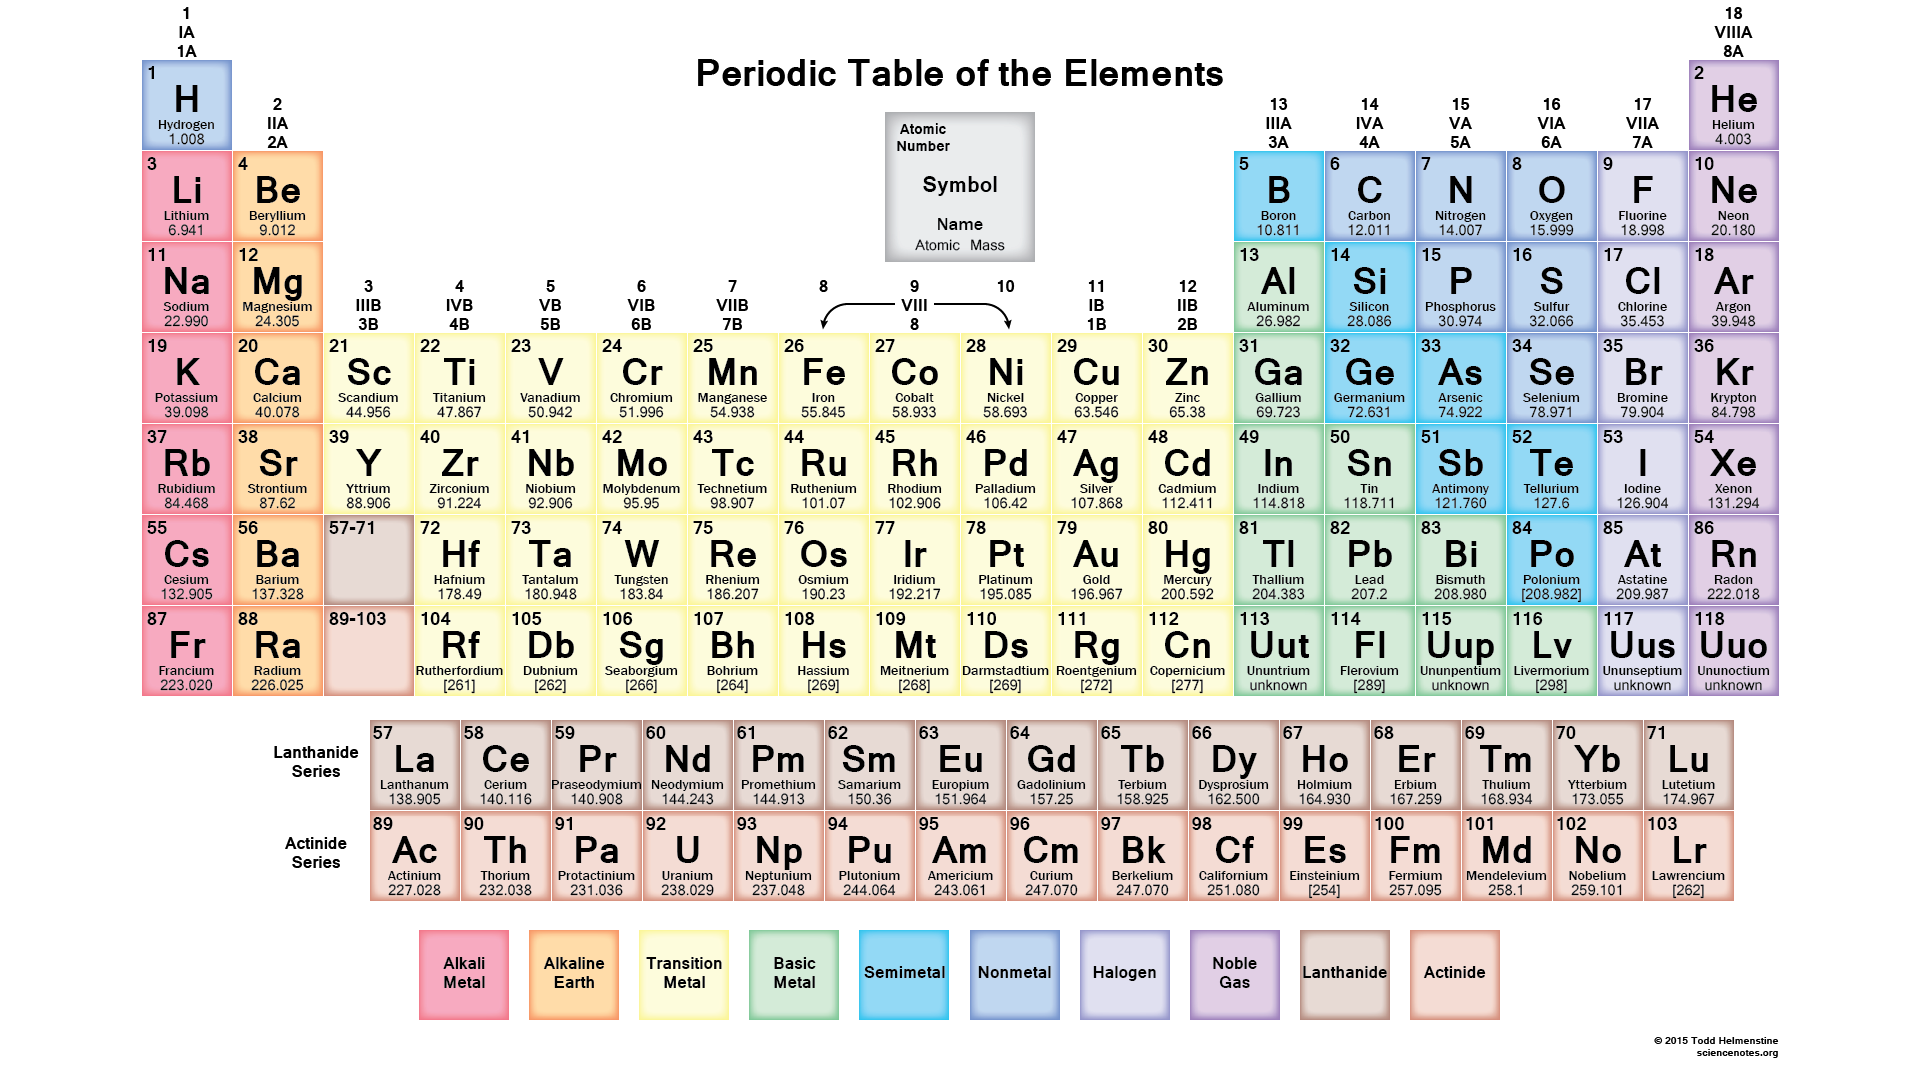
\includegraphics[width=.9\linewidth]{./figs/PeriodicTableMuted.png}


\section{Material balances}
\label{sec-3}
\begin{itemize}
\item general balance
\end{itemize}
\begin{framed}
output = input + generation - consumption - accumulation
\end{framed}

\begin{itemize}
\item Reaction progress
\end{itemize}
\begin{equation*}
n_{j} = n_{j0} + \nu_{j} \xi
\end{equation*}

\begin{itemize}
\item \emph{conversion}
\end{itemize}

\[X_{j} = \frac{n_{j0}-n_{j}}{n_{j0}} = -\frac{\nu_{j}\xi}{n_{j0}} \]

\begin{itemize}
\item Multiple reactions
\end{itemize}

\[ n_{j} = n_{j0} + \sum_{i} \nu_{ij} \xi_{i} \]

\begin{itemize}
\item \emph{yield} \(=n_{j}/n_{j}^{\text{max}}\)

\item \emph{selectivity} (often) defined as amount of desired product over amount of
undesired.
\end{itemize}

\section{Properties of single-phase systems}
\label{sec-4}
\begin{itemize}
\item Ideal solution
\end{itemize}
\[ v \text{ (l/mol)} = \sum_{i} x_{i} v_{i} \]

\[ \frac{1}{\bar{\rho}} = \sum_{i}^{n} \frac{\omega_{i}}{\rho_{i}} \]

\begin{itemize}
\item Ideal gases
\end{itemize}
\[ P V = n R T \text{ or } P v = R T \text{ or } v = \frac{RT}{P} \]

\begin{center}
\begin{tabular}{llll}
R & 8.314472 J / (K mol) & 0.082057 atm l / (K mol) & 1.3806504e-23 J / K\\
\end{tabular}
\end{center}

\begin{itemize}
\item Ideal gas mixture
\end{itemize}
\[ V(N,T,P) = V_{1}(N_{1},T,P) + V_{2}(N_{2},T,P) \]

\[ \frac{P_{1}}{P} = \frac{N_{1} RT/V}{N RT/V} = y_{1}\]

\begin{itemize}
\item van der Waals model
\end{itemize}

\[ P_{\text{vdW}} = \frac{RT}{v-b} - \frac{a}{v^{2}} \]

\[b = v_{c}/3\quad\quad a = \frac{9}{8}R T_{c} v_{c}\]

\begin{itemize}
\item reduced variables
\end{itemize}

\[ T_{r} = T/T_{c}\quad P_{r} = P/P_{c}\quad v_{r}=v/v_{c}\]

\begin{itemize}
\item Soave-Redlich-Kwong (SRK) model
\end{itemize}

\[P_{\text{SRK}} = \frac{RT}{v-b} - \frac{\alpha(T) a}{v(v+b)} \]

\begin{eqnarray*}
a & = & 0.42747 \frac{(R T_{c})^{2}}{P_{c}} \\
b & = & 0.08664 \frac{R T_{c}}{P_{c}} \\
m & = & 0.48508 + 1.55171 \omega - 0.1561 \omega^{2}\\
\alpha & = & \[1+m (1-\sqrt{T_{r}})\]^2
\end{eqnarray*}

\begin{itemize}
\item Pitzer ``acentric'' factor
\end{itemize}

\[\omega = -\log \left ( \frac{P_{sat}}{P_{c}} \right ) \Big|_{T_{r}=0.7} -1 \]

\begin{itemize}
\item Virial expansion
\end{itemize}

\[ P= \frac{RT}{v} \left ( 1 + \frac{B_{2}(T)}{v} + \frac{B_{3}(T)}{v^{2}} + \cdots \right ) \]

\begin{itemize}
\item \emph{compressibility}
\end{itemize}
\[ Z = \frac{P(v,T) v}{RT} \]

\begin{itemize}
\item Law of corresponding states
\[ Z_{c} = 0.27 \]
\end{itemize}

\section{Two-phase systems}
\label{sec-5}

\begin{itemize}
\item Clapeyron equation
\end{itemize}
\[ \frac{d P^{*}}{dT} = \frac{\Delta H_{\text{latent}}}{T(v_{b}-v_{a})} \]

\begin{itemize}
\item Clausius-Clapeyron equation:
\end{itemize}
\[ \ln \frac{P^{*}_{2}}{P^{*}_{1}} \approx -\frac{\Delta H_{\text{vap}}}{R}\left ( \frac{1}{T_{2}} - \frac{1}{T_{1}} \right ) \]

\begin{itemize}
\item Antoine equation
\end{itemize}
\[ \log_{10}P^{*} = A - \frac{B}{T+C} \]

\begin{itemize}
\item Gibbs phase rule
\end{itemize}

\[ DOF = c - \Pi - r + 2\]

\begin{itemize}
\item Raoult's Law
\end{itemize}

\[ x_{A} P^{*}_{A}(T) = P_{A} = y_{A} P \]

\[ P_{\text{bubble}} = \sum x_{i} P_{i}^{*} \]

\[ P_{\text{dew}} = \left ( \sum_{i}\frac{y_{i}}{P_{i}^{*}} \right )^{-1} \]

\begin{itemize}
\item Relative humidity
\end{itemize}

\[ RH(T) = P_{\ce{H2O}}/P^{*}_{\ce{H2O}}(T) \]

\begin{itemize}
\item Henry's Law
\end{itemize}

\[ x_{A} H_{A}(T) = P_{A} = y_{A} P \]

\begin{itemize}
\item Colligative properties
\end{itemize}
\[\Delta T_{b} \approx \frac{R T_{b}^{2}}{\Delta H^{*}_{vap}}x \]

\[\Delta T_{m} \approx \frac{R T_{m}^{2}}{\Delta H^{*}_{m}}x \]

\section{Energy balances}
\label{sec-6}
\begin{itemize}
\item Energy types
\[ E_{K} = \frac{1}{2} m v^{2}\quad\quad \dot{E}_{K} = \frac{1}{2}\dot{m} u^{2} \]

\[ E_{V} = m g h \quad\quad \dot{E}_{V} = \dot{m} g z \]

\[ U = U(T,P,x_{i})\quad\quad H=U+PV\]

\item Closed, constant volume system

\[ \Delta U + \Delta E_{K} + \Delta E_{V} - q - w = 0 \]

\item Open system at steady-state
\end{itemize}

\[ \Delta\dot{H} + \Delta\dot{E}_{K} + \Delta{E}_{P} = \dot{q} + \dot{W}_{s} \]

\begin{itemize}
\item Bernoulli equation:
\end{itemize}

\[ \frac{1}{2} \Delta u^{2} + g\Delta z  + \frac{1}{\rho}\Delta P = 0\]

\section{Energy balances on non-reactive systems}
\label{sec-7}
\begin{itemize}
\item heat capacity
\end{itemize}

\[ C_{v}(T) = \left ( \frac{\partial\hat{U}}{\partial T} \right )_{v} \]

\[ C_{p}(T) = \left ( \frac{\partial\hat{H}}{\partial T} \right )_{p} \]

\begin{itemize}
\item For liquids and solids, \(C_{p} \approx C_{v}\)
\item For ideal gas, \(C_{p} = C_{v} + R\)
\end{itemize}

\section{Energy balances on reactive systems}
\label{sec-8}
\begin{itemize}
\item Reaction energy
\end{itemize}

\[ \Delta H^{\circ}_{r} = \sum_{j} \nu_{j} \Delta \hat{H}_{f,j}^{\circ} \]


\begin{itemize}
\item ``Heat of reaction'' method
\end{itemize}

\[ \Delta \dot{H} = \xi\Delta\hat{H}^{\circ}_{r} + \sum_{out}\dot{n}_{out}\hat{H}_{out}-\sum_{in}\dot{n}_{in}\hat{H}_{in} \]

\[ \Delta \dot{H} = \sum_{i}\xi_{i}\Delta\hat{H}^{\circ}_{r} + \sum_{out}\dot{n}_{out}\hat{H}_{out}-\sum_{in}\dot{n}_{in}\hat{H}_{in} \]

\begin{itemize}
\item ``Heat of formation'' method
\end{itemize}

\[ \Delta \dot{H} = \sum_{out}\dot{n}_{out}\hat{H}_{out}-\sum_{in}\dot{n}_{in}\hat{H}_{in} \]


\section{Transient processes}
\label{sec-9}
\begin{itemize}
\item General balance around any system or element of a system
\end{itemize}

\[ \dot{F}_{out}(t) = \dot{F}_{in}(t) + r(t) - \frac{dF}{dt} \]
% Emacs 25.0.50.1 (Org mode 8.2.10)
\end{document}